\chapter{极限}

\section{定义}
\label{def-limit}

\begin{definition}
    \label{def:limit}
    Let f be a function defined \emph{on some open interval that contains the number $a$}, 
    except possibly at $a$ itself$a$ itself.
    Then we say that the \textbf{limit of } $f(x)$ 
    \textbf{as $x$ approaches $a$ is $L$}, 
    and we write 
    \[
        \lim_{x \to a} f(x) = L
    \]
    if for every number $\varepsilon > 0$ there is a number $\delta > 0$ s.t.
    \[
        0 < |x - a| < \delta \quad \Rightarrow \quad |f(x) - L| < \varepsilon
    \]
\end{definition}
上述定义文本中 
\emph{on some open interval that contains the number} 非常重要。
就考研数学,题目会喜欢给出某点处的导数值,
但是这并不是该点邻域有函数定义的充分条件,
不满足极限定义的要求。

不满足这一点,针对某一些依赖极限的定义定理或者推论则\textbf{不再成立}。
比如给出某一点$n$阶导数值,并不能说明该函数$n$阶可导。
进而 L'Hospital 法则不再成立
\footnote{如例题\ref{counter-example-of-usage-of-L-Hospital}.}。

定义中的 $L$ 是一个常数,
或者说是一个与函数 $f(x)$ 的任何函数参数(如$x$)
无关的表达式\footnote{一个常数也构成我所说的表达式}。
那么,函数极限趋于无穷,则是极限不存在的一种情况。
在相关的概念考察题目中要注意这一点。
如 \cite[question 123]{w660}.

求极限的过程会把一种极限类型转化为另一种。
请在实际做题的时候主义当前的极限类型,并选择最合适的做法,灵活运用。
使用导数定义求极限请参考下一章。

和定积分有关的极限问题请参见
\ref{limit-questions-involved-definite-integral}.

\section{通用技术}

本节将会对下文将会详细描述的各种求极限类型所用到的
一些通用手段进行总结和归纳。 原则上这些内容应当背熟用熟练。

对于所有题型,这些方法都适合。但是对于选择填空题,要应用更多的应试策略。
比如带入选项,或者是通过题目条件举出特殊函数的例子等。

根据极限的定义可知
\[
    \lim_{x \to a^-} f(x) = \lim_{x \to a^+} f(x) = L 
    \Rightarrow 
    \lim_{x\to a} f(x) = L
\]
因此在处理某些初等函数的时候就不得不注意了
\begin{example}
    \cite[page 9]{yc}
    \[
        \lim_{x \to 1} \dfrac{x^2 - 1}{x-1} e^{\frac{1}{x-1}}
    \]
    式子中出现 $e^{\frac{1}{x-1}}$ 则需要注意分类讨论
    \begin{align*}
        \lim_{x \to 1^+} \dfrac{x^2 - 1}{x-1} e^{\frac{1}{x-1}} &= +\infty\\
        \lim_{x \to 1^-} \dfrac{x^2 - 1}{x-1} e^{\frac{1}{x-1}} &= 0
    \end{align*}
    则极限不存在,且不等于 $\infty$.
\end{example} 

\subsection{L'Hospital}

应用 L'Hospital 法则求极限的时候,
要注意极限中有关函数的可导性到多少阶有效。
$n$ 阶可导\textbf{不代表} $n$ 阶导函数存在,
也\textbf{不能保证}$n$阶导函数连续。
因此对有可导阶数有规定的情况,L'Hospital 只能应用到 $n-1$ 阶。
另外也要注意,连续不代表可导
\footnote{参考例子\ref{example-limits-and-varidic-limits-integral-2}}。

参见小节\ref{general-technics-single-var-differentiation}.

\subsection{选择题策略}

使用排除法的时候请务必将每一个选项都试一试,这样可以保证没有漏选。

\subsection{等价无穷小}  \label{super-small}
所有等价无穷小替换都可从 Maclaurin's series 推导出来。

等价无穷小可以在符合一定条件的加减项上使用,
可以在因子上使用。
但是不能在指数上使用(考研数学不建议,是否可用之判断比较复杂)。

\begin{figure}
  \centering
  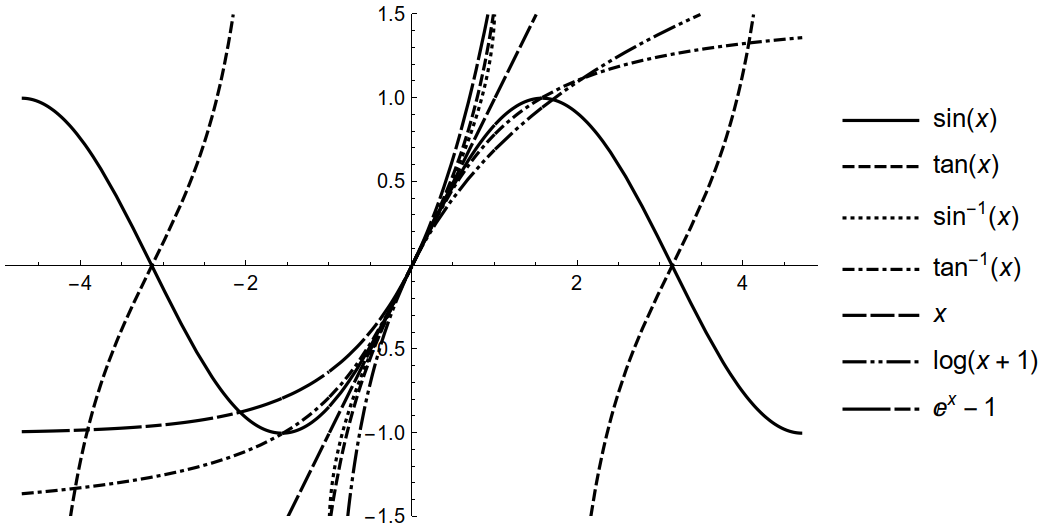
\includegraphics[width=0.5\textwidth]{figure/lots-functiuons-like-x-near-0.png}
  \caption{Lots functions which behaviour near the origin point are like the $x$.}
  \label{fig:example}
\end{figure}

\subsubsection{公式}
这部分等价无穷小可以通过他们的函数图像辅以记忆,
由于等价无穷小是在讨论无限接近于0点的函数状态,
因此要格外关注函数在0点附近性态。

\begin{lemma}[等价无穷小]
	\begin{align}
		x&\sim\sin{x}\sim\tan{x} \\ 
		&\sim\arcsin{x}\sim\arctan{x} \\
		&\sim\ln{(1+x)}\sim e^x-1
	\end{align}
\end{lemma}

还有一组常用公式是从 Maclaurin's series 推导而来的,
作为\textbf{常用结论}使用:
\begin{lemma}[等价无穷小]
	\begin{align}
		x - \sin{x}     &\sim \frac{x^3}{6} \label{rep1} \\
        1 - \cos{x}     &\sim \frac{1}{2} x^2 \\
		\tan{x} - x     &\sim \frac{x^3}{3} \label{rep2} \\
		x - \ln{(1+x)}  &\sim \frac{x^2}{2} \\
		\arcsin{x} - x  &\sim \frac{x^3}{6} \label{rep3}\\
		x - \arctan{x}  &\sim \frac{x^3}{3} \label{rep4}\\
        (1+x)^\alpha-1  &\sim \alpha x \label{rep5}
	\end{align}
\end{lemma}
上述公式\eqref{rep3}和\eqref{rep4}可由
\eqref{rep1}和\eqref{rep2}分别通过项的等价代换得来,
因为他们代换后两项(加减号两边)不等价。
公式 \ref{rep5} 在题目中可能表现为根式的形式,
这种情况可以参考例子
\ref{ex:limit-simplify-and-sqrt-substitution-example-1}
和下面的例子

\begin{example}
    \label{ex:sqrt-substitution-example-2}
    \[
        L = \lim_{x \to 0} \dfrac{\cos 2x - \sqrt{\cos 2x}}{x^k} = a \neq 0
    \]
    求 $k, a$.

    \cite[question 131]{w660}.

    解1\footnote{我自己想到的解法,确实是一件值得高兴的事。2023年10月28日\, 10:55.}:
    \begin{align}
        L &= \lim_{x \to 0} \dfrac{ 1- \cos 2x + \sqrt{\cos 2x} -1 }{-x^k} \notag \\
          &= \lim_{x \to 0} \dfrac{ \dfrac{1}{2} (2x)^2 + \sqrt{\cos 2x} - 1 }{-x^k} \notag \\ 
          &= \lim_{x \to 0} \dfrac{ 2x^2 + \sqrt{1 - 2\sin^2 x } - 1 }{-x^k} \label{eq:rep5-expamle} \\
          &= \lim_{x \to 0} \dfrac{ 2x^2 + \dfrac{1}{2} (-2 \sin^2 x) }{-x^k} \notag \\
          &= \lim_{x \to 0} \dfrac{ x^2 }{-x^k} = -1 \notag
    \end{align}
    则 $k = 2, a = -1$.

    步骤 \ref{eq:rep5-expamle} 利用了式子 \ref{rep5}.
\end{example}

\subsubsection{何时可用?}

除了我们熟悉的式子中的\textbf{因子可以直接使用}等价无穷小代换之外,
实际上因子中的\textbf{项}也可以。但是有条件:
\textbf{替换后两项不能等价\footnote{相等 $\Rightarrow$ 等价,反之不成立。}。}比如:
\[
    \lim_{x \to 0} \frac{\sin{x} - \tan{x} }{x^3} \neq 0
\]
中LHS的分子中不可以将两个项替换成$x$,因为 $x$ 显然和 $x$ 等价.
换句话说,我们不让相加减的两个函数的 Tylor Expantion 中的第一项
(所谓的等价无穷小量)消去即可。即:
\begin{align}
	\lim_{ x\to x_0 } \frac{a_1}{a_2} &\neq 1  &\Rightarrow a_1 - a_2 \sim b_1 - b_2 \\
	\lim_{ x\to x_0 } \frac{a_1}{a_2} &\neq -1 &\Rightarrow a_1 + a_2 \sim b_1 + b_2
\end{align}
这种利用等价无穷小甚至是Tylor公式代换后,项等价的例子可以参考
\cite[question 130]{w660},其中官方题解首先对式子进行一种特殊的化简,
值得参考。
若替换的因子或者项出现在分式中,要注意需要分子分母上下同阶。
否则不能替换,请参考例子\ref{ex:super-small-wrong-usage-example-1}。

另外,\emph{无穷小代换本质上是 Tylor 公式
\footnote{参见小节\ref{tylor}}的一个化简的应用\footnote{令人反感的应试的产物!}。}
在加减式子中利用无穷小代换是需要格外注意不能出现
两项等价抵消的,这种抵消的现象是错误。不同的函数
的Tylor公式展开也许第一项都是 $x$,但是后续的项
却不同。然而等价无穷小替换却只关心到了第一项。
在使用等价无穷小代换的过程中如果感到不放心,
可以查看一下对应的Tylor展开式。

\begin{example}
    \label{ex:super-small-wrong-usage-example-1}
    设
    \[
        L_1 = \lim_{x \to 0} \dfrac{\sin 6x - (\sin x) f(x)}{x^3} = 0
    \]
    求值 
    \[
        L_2 = \lim_{x \to 0} 
        \dfrac{
            \overbrace{
                6 - f(x)
            }^{\mathclap{\mbox{需要在$L_1$的变形中体现这个式子}}}
        }{x^2}
    \]

    \cite[question 135]{we}.

    本题目不能使用等价无穷小代换(如$\sin 6x \sim 6x$),
    纵使分子在替换完后两个项不等价。
    原因是分子分母不同阶,分母是3阶而分子是1阶。
    所谓的等价无穷小代换只是Tylor展开
    \footnote{请参见小节\ref{tylor}}的第一项
    \footnote{毫无疑问是1阶的,那么请问展开的其他项的系数去哪里了?}。
    如果分子分母都是1阶的,则替换是没有问题的。
    如果说我们就是想等价无穷小替换,则需要将分子的阶数升高
    \begin{equation}
        \label{eq:3-order-super-small-substitution-instance-1}   
        x- \sin x \sim \frac{1}{6} x^3
    \end{equation}
    那么
    \begin{align*}
        L_1 &= \lim_{x \to 0} 
                \dfrac{
                    \sin(6x) 
                    \overbrace{
                        -6x + 6x
                    }^{\mathclap{\mbox{加减项}}}-(\sin x)f(x)
                }{x^3} \\[1em]
            &= \dfrac{
                \splitfrac{
                    \sin(6x) -6x +6x 
                }{
                    + \underbrace{
                        6 \sin x- (\sin x)f(x)
                    }_{\mathclap{\mbox{为了凑$6-f(x)$}} } - 6 \sin x
                }
            }{x^3} = L_3 \\[1em]
            &=  \lim_{x \to 0} 
                \dfrac{\overbrace{\sin 6x - 6x}^{\mathclap{
                    \mbox{
                        与分母阶数保持相同
                    }
                }}}{x^3} 
                +  \lim_{x \to 0} \dfrac{6x - \sin 6x}{x^3} \\
            &\quad + \underbrace{\lim_{x \to 0} \dfrac{(6 - f(x)) \sin x}{x^3}}_{L_2} \\
            &= 0 = -36 + 1 + L_2
    \end{align*}
    解得 $L_2 = 35$.

    660给出两个解答方案:
    \begin{align*}
        L_3 &= \underbrace{\lim_{x \to 0} \dfrac{\sin 6x - 6 \sin x}{x^3}}_{A} + 
               \lim_{x \to 0} \left[\dfrac{\sin x}{x} \cdot \dfrac{2 - f(x)}{x^2}\right] \\
            &= 0
    \end{align*}
    则有
    \begin{equation}
        \label{eq:when-super-small-substitution-could-be-used-rep-1}
        L_2 = -A = \lim_{x \to 0} \dfrac{6 \sin x - \sin 6x}{x^3}
    \end{equation}
    \begin{itemize}
        \item 方法一,
            直接在式子
            \ref{eq:when-super-small-substitution-could-be-used-rep-1} 
            上使用 L'Hospital 法则;
        \item 方法二,
            用Tylor公式
            \footnote{也可以避开分子分母不同阶的陷阱。参见小节\ref{tylor}。}。
    \end{itemize}
\end{example}

\subsubsection{定积分中的替换}
\label{limit-rerepresenting-in-variable-limits-integral}
设置 $f(x)$ 和 $g(x)$ 在某邻域连续,
并且$\lim_{x \to 0} \frac{f(x)}{g(x)} = 1$
那么
\begin{equation}
	\int_0^{x} f(t) dt \sim \int_0^{x} g(t) dt
\end{equation}
如果$g(x)=c$也是可以使用本结论的,请不要忽视这一重要用途。For example:
\[
\int_0^x e^{t^2} dt \sim \int_0^{x} 1 dt
\]

还有\textbf{更一般}的情况:
\begin{lemma}
	Suppose $f(x)$ and $g(x)$ are continuous on 某邻域,and $\lim_{x \to a} \frac{f(x)}{g(x)} = 1$ 
	Thus, 
	\begin{equation}
		\int_a^{x} f(t) dt \sim \int_a^{x} g(t) dt
	\end{equation}
\end{lemma}

\subsection{Lagrange Mean Value Theorem} \label{lagrange-limit}
当极限式子中某部分出现两个函数相减的形式,就可使用这种方法化简。
其中析出的一个 $\xi$ 往往可以通过极限趋向来确定,
作为非零因子\ref{non-zero-factor}算出。

当 $x\to0$的时候,如果析出的函数导数是 $e^{\xi} = 1$ 那么,不难理解有
\begin{equation}
	e^{\alpha(x)} - e^{\beta(x)} \sim \alpha(x) - \beta(x)
\end{equation}
其中 $\alpha(x) \to 0$ 且 $\beta(x) \to 0$,
但是这个结论\textbf{考研不能直接使用!}

\section{其他重要结论}
\begin{lemma}
	\begin{equation}
		\lim_{n \to \infty} \sqrt[n]{a^{n}_{1} + a^{n}_{2} + 
        \cdots + a^{n}_{n}} = \max_{1\leq i \leq n}{\sqrt{a_{i}^{n}}}
	\end{equation}
\end{lemma}

\begin{lemma}
    \begin{equation}
        \frac{0}{()} \to c \Rightarrow () \to 0
    \end{equation}
    which $c$ is a constant number.
    同理
    \begin{equation}
        \frac{()}{0} \to c \Rightarrow () \to 0
    \end{equation}
    which $c$ is a constant number.
\end{lemma}

\begin{lemma}
    \[
        \lim_{x \to 0^+} x^{\alpha} \ln^{\beta}x = 0
    \]
    Once $a$ is a positive number. ??? %TODO
\end{lemma}

\section{极限之 Squeeze Theorem 还是 定积分定义?}
\label{use-squeeze-or-definition-of-integral}

观察数列求和式子中每一项的分母,找到其中的\textbf{变化部分和不变部分}。
两部分若具有不同的数量级则使用 Squeeze Theorem;
两部分若具有相同的数量级则使用 定积分定义
\footnote{
    参见 Definition\ref{defination-definite-integral},
    和 Equation\ref{eq:the-other-definition-definite-integral}.
}。

\begin{example}
    \begin{equation} \label{eq:example-squeeze}
        \lim_{n \to 0} \left[ 
        \dfrac{n}{n^2+1} + \dfrac{n}{n^2+2} + \cdots + \dfrac{n}{n^2+n} 
        \right]  
    \end{equation}
    \begin{equation} \label{eq:example-defination-int}
        \lim_{n \to 0} \left[ 
        \dfrac{n}{n^2+1^2} + \dfrac{n}{n^2+2^2} + \cdots + \dfrac{n}{n^2+n^2} 
        \right]  
    \end{equation}
    本例子中\ref{eq:example-squeeze}各项分母中的两项里面
    \textbf{不变的部分为$n^2$,变化的部分是$1,2,3,4,\cdots$}.
    两部分具有\textbf{不同数量级},这种情况使用\textbf{Squeeze Theorem}。

    本例子中\ref{eq:example-defination-int}各项分母中的两项里面
    \textbf{不变的部分为$n^2$,变化的部分是$1^2,2^2,3^2,4^2,\cdots$}.
    两部分具有\textbf{相同数量级},
    这种情况使用\textbf{定积分定义}

    那么针对使用定积分解决的问题,
    我们接下来提一个因子
    \footnote{
        被武忠祥老师称为“可爱因子”, 事实上由 
        $\Delta x$变形而来, 
        参见 Equation \ref{eq:the-other-definition-definite-integral}
    },这样可构造出黎曼和定积分定义:
    \begin{equation*}
        \lim_{n \to 0} \dfrac{1}{n} \left[ 
        \dfrac{1}{1+\left(\dfrac{1}{n}\right)^2} + 
        \dfrac{1}{1+\left(\dfrac{2}{n}\right)^2} + \cdots + 
        \dfrac{1}{1+\left(\dfrac{n}{n}\right)^2}
        \right]  
    \end{equation*}
    这样 $f(x) = \dfrac{1}{1+x^2}$
    \begin{equation*}
        \mbox{LHS} = \int_{0}^{1} \dfrac{1}{1+x^2} dx = \pi / 4
    \end{equation*}
\end{example}

\begin{example}
    \label{ex:squeeze-theorm-example-1}
    \begin{align*}
        &\splitfrac{
            \lim_{n \to \infty} \left(
            \dfrac{1}{n^2 + n + 1} + 
            \dfrac{2}{n^2 + n + 2} + 
            \right.
        }{
            \left.
            \dfrac{3}{n^2 + n + 3} + 
            \cdots + 
            \dfrac{n}{n^2 + n + n}
            \right)
        } \\
        = &\lim_{n \to \infty} \sum_{i = 1}^n \dfrac{i}{n^2 + n + i}
    \end{align*}

    \cite[question 137]{w660}.
    
    因为   
    \begin{equation}
        \label{eq:inequality-squeeze-example-1}
        \sum_{i = 1}^{n} \dfrac{i}{n^2 + n + n} \leq 
        \sum_{i = 1}^{n} \dfrac{i}{n^2 + n + i} \leq 
        \sum_{i = 1}^{n} \dfrac{i}{n^2 + n + 1}
    \end{equation}
    所以
    \[
        \dfrac{\sum_{i = 1}^n i}{n^2 + n + n} \leq 
        \sum_{i = 1}^{n} \dfrac{i}{n^2 + n + i} \leq 
        \dfrac{\sum_{i = 1}^n i}{n^2 + n + 1}
    \]
    而
    \begin{align*}
        &\lim_{n \to \infty} \dfrac{\sum_{i = 1}^n i}{n^2 + n + n} 
        =\lim_{n \to \infty} \dfrac{\frac{1}{2} n(n + 1)}{n^2 + n +n} 
        =\dfrac{1}{2}\\
        &\lim_{n \to \infty} \dfrac{\sum_{i = 1}^n i}{n^2 + n + 1} 
        =\lim_{n \to \infty} \dfrac{\frac{1}{2} n(n + 1)}{n^2 + n +1} 
        =\dfrac{1}{2}
    \end{align*}
    由 Squeeze Theorem, $\text{LHS} = 1/2$.
\end{example}

\subsection{Squeeze Theorem 的放缩法}

三步走策略\footnote{引用自\url{https://zhuanlan.zhihu.com/p/596173443}}:
\begin{enumerate}
    \item 写巨算符\footnote{参见小节\ref{giant-operator}}求和的形式
    \item 找出影响最小的项
    \item 对这个项进行放缩
\end{enumerate}

例子 \ref{ex:squeeze-theorm-example-1} 
中的所谓影响最小的项就是\emph{分母中的}$i$,
对该项进行放缩,选取原式子中该项位置最大和最小值,
则有步骤(不等式)\ref{eq:inequality-squeeze-example-1} 两个。

\section{0/0型}
\label{0-slash-0-type-limits}
\subsection{常用方法}
\begin{enumerate}
    \item L'Hospital \footnote{注意可导性陷阱,参见小节\ref{def-limit}.}
	\item 等价无穷小代换 \ref{super-small}
	\item Tylor 公式
	\item 加减项(若上述方法均不方便)
        \footnote{武讲义0/0例3,三星笔记求极限通法2P10}
\end{enumerate}

这种类型的极限之所以不好求,
是因为分母有0因子。
则将分母上的0因子消掉,也是一个很好的办法。

加减项可参考本例:
\begin{example}
    \begin{align*}
        &\lim_{x \to 0} \dfrac{\arcsin{x} - \sin{x}}{\arctan{x} - \tan{x}} \\
        = &\lim_{x \to 0} \dfrac{(\arcsin{x} -x) - (\sin{x}-x)}{(\arctan{x}-x) - (\tan{x}-x)}
    \end{align*}
    然后使用无穷小替换
    \ref{super-small}快速求解
    \footnote{结果是 $-1/2$,本题目也可使用麦克劳林级数替换}。
\end{example}

\subsection{原式化简}
\begin{enumerate}
	\item 非零因子(fator)先求出 \label{non-zero-factor}
	\item 有理化
	\item 变量代换
\end{enumerate}

其中,往往在有理化过程后出现非零因子,这个时候请立刻将非零因子求出,
提到式子外面。比如:

\begin{example}
    \label{ex:limit-simplify-and-sqrt-substitution-example-1}

    \begin{align*}
        &\lim_{x \to 0} \dfrac{\sqrt{1+\tan{x}} - \sqrt{1+\sin{x}}}{x \ln{(1+x)} - x^2} \\
        =&\lim_{x \to 0} \dfrac{\tan{x} - \sin{x}}{x \ln{(1+x)} - x^2} \cdot
        \underbrace{\dfrac{1}{\sqrt{1+\tan{x}} + \sqrt{1+\sin{x}}}}_{\mbox{非零因子}}\\
        =&\dfrac{1}{2} \dfrac{\tan{x} - \sin{x}}{x \ln{(1+x)} - x^2}
    \end{align*}
    例题选自武忠祥强化课程,本题目接下来可以通过
    \textbf{拉格朗日中值定理}\footnote{参考\ref{thm:lagrange}}来求解。
    详情请参考求极限通法2 三星笔记。

    本题分子里面含有根号,实际上也就是开 $1/2$ 次方,这种情况还可以构造
    $(1+x)^\alpha - 1 \sim \alpha x$
    \ref{super-small}
    \begin{equation*}
        \mbox{LHS} = \lim_{x \to 0}
        \dfrac{\sqrt{1+\sin{x}}\left[ 
            \sqrt{1+\dfrac{\tan{x}-\sin{x}}{1+\sin{x}}}	- 1
            \right] }{x \ln{(1+x)} - x^2}
    \end{equation*}
\end{example}

\section{无穷比无穷}

\subsection{常用方法}

\begin{enumerate}
    \item L'Hospital \footnote{当心可导陷阱,参见小节\ref{def-limit}}
	\item “抓大头”
        \footnote{大题必须要写好步骤,必须要体现分母无穷大于分子}
\end{enumerate}

\section{1 to Infinity}
\subsection{常用方法}
\begin{enumerate}
	\item 凑基本极限
	\item 改写成指数
	\item 应用常用结论
\end{enumerate}

其中常用结论可以精炼为下面三步:
\begin{enumerate}
	\item 写标准型,令
	\[\mbox{LHS} = \lim{} \left[ 1+\alpha(x)\right] ^{\beta(x)}\]
	其中 \[\alpha(x)\to0, \beta(x)\to\infty\]
	\item 求极限 $A = \lim \alpha(x)\beta(x)$
	\item 写结果 $\mbox{LHS} = e^{A}$
\end{enumerate}

\cite[question 30]{w660}.

\begin{example}
    \label{counter-example-of-usage-of-L-Hospital}
    设 $f(x)$ 在 $x = 0$ 可导且 $f(0) = 1, f'(0) = 3$,
    则
    \[
        L = \lim_{n \to \infty} {\left[
            f \left(\dfrac{1}{n}\right) 
        \right]}^{\left(\dfrac{\frac{1}{n}}{1 - \cos \frac{1}{n}} \right)}
    \]
    \cite[question 30]{w660}.

    令 $t = 1/n$,有 $t \to 0$.
    \begin{align*}
        L &= \lim_{t \to 0} {f(t)}^{\dfrac{t}{1 - \cos t}} 
          = \lim_{t \to 0} {f(t)}^{\dfrac{t}{\frac{1}{2} t^2}}\\
          &= \lim_{t \to 0} {f(t)}^{\frac{2}{t}} 
          = \lim_{t \to 0} {[1 + (f(t) - 1)]}^{\frac{2}{t}}
    \end{align*}
    有(\textbf{典型错误!})
    \begin{align}
        &\lim_{t \to 0} (1+f(t)) \frac{2}{t} \notag \\
        = &2\lim_{t \to 0} \dfrac{1+ f(t)}{t} 
        = 2\lim_{t \to 0} {f'(t)} \label{eq:example-L-Hospital-illegal-usage}  \\
        = &6 \notag
    \end{align}
    所以
    \[
        L = e^{6}
    \]
\end{example}

上面的错误例子中步骤(\ref{eq:example-L-Hospital-illegal-usage})使用
L'Hospital法则求极限。但题目只保证了 $x = 0$ 点处可导,
并且给出了该点处导数值。 但给出的条件并不符合导数的定义
\footnote{参见 Definition\ref{def:single-order-derivative}.}
对极限存在的要求,仅仅给出某一点处导数值并不能说明该点临域函数有定义。

\section{确定求极限式子里的参数}

这种题目就是要将其按照正常极限进行求解,
在求的过程中或者是最后得到要求的参数。

\begin{lemma} \label{lm:inf-zero-zero}
	\begin{equation}
		\infty \cdot () \to 0 \Rightarrow () \to 0
	\end{equation}

\end{lemma}

例题:
\[
\lim_{x \to -\infty} \sqrt{x^2+x+1} +  ax + b = 0
\]
求 $a, b.$
这道题我们可以首先提出一个 $x$,这样就可以构造 \ref{lm:inf-zero-zero}:

\begin{align*}
	&\mbox{LHS} = \lim_{x \to -\infty} \left(\overbrace{-x}^{ \to \infty }\right)
	\left( 
	\underbrace{\sqrt{1+\dfrac{1}{x}+\dfrac{1}{x^2}} + a + \dfrac{b}{x}}_{\to 0}
	\right) = 0\\
	&\therefore 1-a = 0, a = 1.
\end{align*}
进一步就可以轻松求出 $b$.

\section{无穷小阶数比较}

\begin{definition}
    In calculus, an infinitesimal is a concept that refers 
    to an extremely small quantity, approaching zero 
    but not quite equal to zero. It is often denoted 
    by the symbol $dx$ or $dy$ and is used to represent 
    the change in a variable, typically in the context of 
    limits and derivatives.

    Formally, an infinitesimal is defined as a variable that, 
    when it tends towards zero, represents an infinitely 
    small change in a function or a curve. 
    It's a fundamental concept in calculus, 
    particularly in the development of derivatives and integrals, 
    allowing us to understand how functions change at specific points.

    Infinitesimals are a foundational element of calculus and 
    are essential for understanding rates of 
    change and areas under curves, among other mathematical concepts.
\end{definition}

\emph{比较两个无穷小阶的问题就是求 0/0 型极限
    \footnote{参见小节 \ref{0-slash-0-type-limits}.},
}
因此常用的方法就是求 0/0 型极限的常用方法。

三种主要方法:
\begin{enumerate}
    \item L'Hospital \footnote{当心可导陷阱,参见小节\ref{def-limit}}
	\item 等价无穷小代换
	\item Tylor 公式
\end{enumerate}

这三种方法都是用来在构造完 $f(x)/g(x)$ 之后进行约分化简的时候使用的。
考察这种知识点的提醒一般比较集中在选择题。
因此在做题的时候要格外注意策略,不要乖乖按照最一般的直接法生算。
所谓的定义法也就是构造
\[
    \lim_{x\to 0} \dfrac{f(x)}{g(x)}
\]
计算这个极限,看结果是 $\infty, 0$还是$c$。 

\begin{lemma}[L'Hospital求导定阶]
	若 $x \to 0$ 时 $f(x)$ 是无穷小量,
    且 $f'(x)$ 是 $x$ 的 $k(k>0)$ 阶无穷小,
	则 $f(x)$ 是 $k+1$ 阶无穷小。即
	\begin{equation}
		\lim_{x \to 0} \dfrac{f(x)}{x^{n+1}} 
        = 
        \lim_{x \to 0} \dfrac{f'(x)}{(n+1)x^{n}} \neq 0
	\end{equation}
\end{lemma}

求导定阶的目的是通过求导数简化我们关系的函数,
在实际考察中会有函数并不能简单地定阶,则应用求导定阶,
如下例。

\begin{example}
    TODO. %TODO
\end{example}

\begin{lemma}
	若 $f(x)$ 在 $x=0$ 的某邻域内连续,
    而且当 $x\to0$ 时 $f(x)$ 是 $x$的 $m$ 阶无穷小,
	$\sigma(x)$ 是 $x$ 的 $n$ 阶无穷小,则当 $x\to0$ 时
	\begin{equation*}
		F(x) = \int_{0}^{\sigma(x)} f(t) dt
	\end{equation*}
	是 $x$ 的 $n(m+1)$ 阶无穷小
\end{lemma}

\begin{lemma}
	低阶 + 高阶 $\sim$ 低阶
	
	$x \to 0, x^2+x^3 \sim x^2$
\end{lemma}

\begin{example}
    把 $x \to 0^+$ 时的无穷小
    \begin{align*}
        \alpha &= \int_0^x \cos t^2 \mathrm dt, \\
        \beta  &= \int_0^{x^2} \tan \sqrt{t} \mathrm dt, \\
        \gamma &= \int_0^{\sqrt{t}} \sin t^3 \mathrm dt
    \end{align*}
    使排在后面的是前一个的高阶无穷小,则正确的排列方式是什么?
    \cite[page 40, example 1]{we}.

    方法三(求导定阶)
    
    由于
    \[ \begin{dcases*}
        \dfrac{\mathrm d\alpha}{\mathrm dx} = \cos x^2  \to 1 & x \mbox{的0阶无穷小}\\
        \dfrac{\mathrm d\beta }{\mathrm dx} = 2x \tan x \sim 1  & x\mbox{的2阶无穷小}\\
        \dfrac{\mathrm d\gamma}{\mathrm dx} = \dfrac{1}{2 \sqrt{x}} \sin x^{\frac{3}{2}} \sim \dfrac{1}{2}x & \mbox{x的1阶段无穷小}.
    \end{dcases*}\]
    所以,正确的排序是 $\alpha, \gamma, \beta$.
\end{example}

\section{连续定义}

\begin{definition}
	函数某点的极限值和函数值相等,称该函数在该点连续。
\end{definition}
当然也有左右连续,将上述定义中的极限值分别换成左/右极限值,
则左右连续的定义易知。

\section{间断点分类问题}
一般这种题型要求\textbf{讨论}间断点的类型,
则需要写下明确的间断点的位置。 并且对每个间断点的类型进行讨论,
这种讨论必须要对间断点两边分别求极限才可行。
或者那种比较容易判断的\textbf{可去}间断点,则直接求极限。

\begin{itemize}
    \item 第一类间断点
        \begin{itemize} 
            \item 可去间断点
            \item 跳跃间断点
        \end{itemize}
    \item 第二类间断点
        \begin{itemize}
            \item 函数至少有一侧极限不存在的点
        \end{itemize}
\end{itemize}

\begin{example}
    \[
        f(x) = \dfrac{(x+1) | x-1 |}{e^{\frac{1}{x-2}} \ln |x|}
    \]
    的可去间断点的个数是多少?

    \cite[page 46, pdf 57, example 4]{we}.

    根据分母各因子
    \footnote{其中$\ln |x|$可导出两个条件,不要遗漏 $x \neq 0$ 的要求.}
    可看出 $x = 0, x = \pm 1$ 和 $x = 2$ 为 $f(x)$ 的间断点,
    其余处处连续。

    由于
    \[
        \lim_{x \to 0} f(x) = 0
    \]
    因此 $x = 0$ 是可去间断点;
    \begin{align*}
        \lim_{x \to 1} f(x) &= 2e \lim_{x\to 1} \dfrac{|x - 1|}{\ln x} = 2e \lim_{x\to 1} \dfrac{|x - 1|}{x - 1} \\
                            &= 
                            \begin{dcases}
                                2e & x \to 1^+ \\
                                -2e & x \to 1^-
                            \end{dcases}
    \end{align*}
    因此 $x = 1$ 为跳跃间断点;
    \begin{align*}
        \lim_{x \to -1} f(x) &= 2 \sqrt[3]{e} \lim_{x \to -1} \dfrac{1 + x}{\ln |x|} = 2 \sqrt[3]{e} \lim_{x \to -1} \dfrac{1}{\frac{1}{x}} \\
                             &= 2 \sqrt[3]{e}
    \end{align*}
    因此 $x = -1$ 是可去间断点;
    \begin{align*}
        \lim_{x \to 2^+} f(x) = 0, \quad \lim_{x \to 2^-} f(x) = \infty.
    \end{align*}
    因此 $x = 2$ 是第二类间断点。
\end{example}

\section{例题}

\begin{example}
    \begin{align*}
         &\lim_{x \to - \infty} \dfrac{\ln (1+ 3^x)}{\ln (1+ 2^x)} \\
        =&\lim_{x \to - \infty} \dfrac{3^x}{2^x} \\
        =&0
    \end{align*}
\end{example}

\begin{example}
    \begin{align*}
         &\lim_{x \to + \infty} \dfrac{\ln (1+3^x)}{\ln (1+2^x)}\\
        =&\lim_{x \to + \infty} \dfrac{\ln 3^x \left(\dfrac{1}{3^x} + 1\right)}{\ln 2^x \left(\dfrac{1}{2^x} + 1\right)}\\
        =&\lim_{x \to + \infty} 
        \frac{
            x\ln 3 + \ln \left(1+\dfrac{1}{3^x}\right)
        }{
            x\ln 2 + \ln \left(1+\dfrac{1}{2^x}\right)
        }\\
        =&\lim_{x \to + \infty} 
        \frac{
            \ln 3 + \dfrac{\ln \left(1+\dfrac{1}{3^x}\right)}{x}
        }{
            \ln 2 + \dfrac{\ln \left(1+\dfrac{1}{2^x}\right)}{x}
        }\\
        =&\dfrac{\ln 3}{\ln 2}
    \end{align*}

    显而易见的\footnote{如图\ref{fig:ln-1-plus-3-to-x-and-its-sibling}所示。}
    \[
        \lim_{x \to +\infty} f(1 + x) = \lim_{x \to +\infty} f(x)
    \]
    我个人认为在这种比较简单的极限上可以利用这种符合直觉的判断来加速解题,
    只要题目不要求写过程。那么原先的题目就变成了
    \[
         \lim_{x \to + \infty} \dfrac{\ln (1+3^x)}{\ln (1+2^x)} = 
         \lim_{x \to + \infty} \dfrac{\ln (3^x)}{\ln (2^x)}
    \]
\end{example}

\begin{figure}
  \centering
  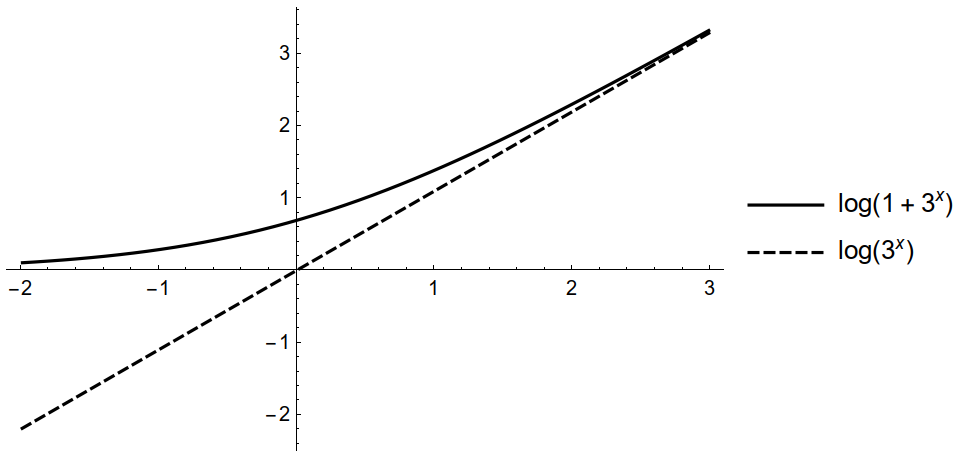
\includegraphics[width=0.5\textwidth]{figure/ln(1plus3tox)-ln(3tox).png}
  \caption{The figure of $\ln(1+3^x), \ln(3^x)$.}
  \label{fig:ln-1-plus-3-to-x-and-its-sibling}
\end{figure}

\begin{example}
    \label{example-limits-and-varidic-limits-integral-1}
    \[
        L = \lim_{x \to 0} 
        \dfrac{\int_{x^2}^{x} \dfrac{\sin (xt)}{t} \mathrm dt }{x^2}
    \]
    不要被积分\footnote{参见章节\ref{single-var-integral}}符号吓到,题目不难发现为$0/0$ 型,
    可以使用 L'Hospital 法则消灭积分符号。那么
    \[
        L = \lim_{x \to 0} \dfrac{2x \dfrac{\sin x^2}{x^2} - 3x^2 \dfrac{\sin x^3}{x^3}}{2x}
    \]
    然后使用无穷小代换等方法解出极限。

    另外,变限积分上下限符号和被积函数符号同时作为一个表达式的因子的时候,
    如本题目的 $\sin (xt)$,则可以使用换元法将两个符号分离
    \footnote{另请参考例\ref{example-limits-and-varidic-limits-integral-2}}:
    \[
        \int_{x^2}^{x}   \dfrac{\sin (xt)}{t}\mathrm dt  = 
        \int_{x^3}^{x^2} \dfrac{\sin s}{s}   \mathrm ds
    \]
    其中 $\mathrm ds = x \mathrm dt$.
\end{example}

